\documentclass[journal]{IEEEtran}
\usepackage[utf8]{inputenc}
\usepackage[T1]{fontenc}
\usepackage{graphicx}
\usepackage{booktabs}
\usepackage{amsmath}
\usepackage{amssymb}
\usepackage{textcomp}
\usepackage[hidelinks]{hyperref}
\usepackage{tikz}
\usetikzlibrary{positioning,arrows.meta}
\renewcommand{\ttdefault}{cmtt}

\graphicspath{{figures/}}

\begin{document}

\title{Foundation Brain: A Task-Agnostic Contrastive Pretraining Backbone for Simultaneous EEG and fNIRS}

\author{Anonymous Authors}

\markboth{INDICON 2026 Submission}{Anonymous Authors: Foundation Brain}

\maketitle
\thispagestyle{empty}
\pagestyle{empty}

\begin{abstract}
Brain-computer interfaces combine two complementary types of brain recordings -- one capturing fast electrical activity, the other slower changes in blood oxygen -- to recognize what a person is thinking or doing. Existing systems of this kind must be built and trained from scratch for every new mental task, much like computer-vision models before general-purpose pretraining became standard. Foundation Brain is introduced here as a pretraining approach that learns a single, general-purpose representation of combined brain-signal data without ever being told which mental task a recording belongs to. Instead, the system is taught to recognize when two simultaneously recorded signals came from the same moment in time. This representation is evaluated by freezing it and attaching only a lightweight classifier on top, comparing against a fully supervised, task-specific baseline. On a word-generation task, across 11 subjects, the frozen representation reaches 0.632 accuracy (0.618 F1), close to the fully supervised baseline's 0.671 accuracy (0.660 F1), despite never seeing task labels during pretraining. The baseline's originally reported numbers are also reproduced under several evaluation setups to ensure a fair comparison. Most importantly, whether a representation learned from one mental task transfers to a different one it never saw during training is tested. Probing on a three-class working-memory task, after pretraining only on word generation, reaches 0.381 accuracy against a 0.333 chance level -- early evidence that a single general-purpose brain-signal representation could replace multiple task-specific models.
\end{abstract}

\section{Introduction}
Electroencephalography (EEG) offers millisecond-scale temporal resolution of cortical electrical activity. Functional near-infrared spectroscopy (fNIRS) offers complementary, slower hemodynamic (blood-oxygenation) signals with better spatial localization. Combining the two modalities has been shown to improve classification accuracy across cognitive tasks ranging from working-memory load to motor imagery. However, every published EEG+fNIRS architecture known to the authors -- including EF-Net, STA-Net, and DC-AGIN -- is trained end-to-end for one specific downstream task. There is no published EEG+fNIRS model that produces a reusable, task-agnostic embedding evaluated across heterogeneous downstream tasks.

This gap mirrors the pre-foundation-model era of computer vision and language modeling. In that era, every new task required a model trained from scratch. This was true prior to the adoption of self-supervised pretraining followed by lightweight task-specific probing. The Contrastive Language-Image Pretraining (CLIP) paradigm~\cite{radford2021} is adapted here to align EEG and fNIRS embeddings of the same simultaneously recorded brain state; CLIP was originally designed to align image and text embeddings. The underlying hypothesis is that a backbone trained purely to recognize \emph{that this EEG window and this fNIRS window came from the same moment in the same trial} will, as a side effect, learn representations of brain state that are useful for downstream cognitive-state classification. This should hold true without the backbone ever seeing a single task label during pretraining.

The contribution of this work is fourfold. (1) A symmetric InfoNCE pretraining objective and dual ShallowConvNet-style encoder architecture is introduced for paired EEG+fNIRS windows. (2) A leave-one-subject-out (LOSO) evaluation is presented, showing the frozen backbone's linear-probe performance is competitive with a fully-supervised baseline on the task it was pretrained on. (3) A faithful reproduction of the supervised baseline's modality ablations and subject-dependent setting is provided, isolating which evaluation regime each reported number belongs to. (4) A direct cross-task transfer experiment is conducted -- pretraining on one cognitive task and linearly probing on an entirely different one -- which is, to the authors' knowledge, the first reported test of task-agnostic transfer for a jointly-trained EEG+fNIRS backbone.

\section{Background and Related Work}
EF-Net (used here as the supervised baseline) is a dual-branch CNN~\cite{arif2024}. Separate convolutional towers process EEG and fNIRS as 2D arrays (channels $\times$ time), are projected to fixed-size vectors, concatenated, L2-normalized, and passed through a classification head, trained end-to-end with cross-entropy for one specific task. STA-Net~\cite{liu2025} introduces cross-attention alignment layers (fNIRS-guided Spatial Alignment and EEG-guided Temporal Alignment) that fuse modalities inside the network, but, like EF-Net, produces no reusable intermediate embedding -- the fused representation only exists as an internal activation of a single-task model.

DC-AGIN~\cite{yu2026} follows the same pattern for cross-subject emotion recognition, combining an attention-weighted graph isomorphism encoder with a cross-modal contrastive fusion module, and a hybrid EEG+fNIRS motor-imagery architecture in the same vein is given by Xu et al.~\cite{xu2023}. None of these architectures separate representation learning from task-specific supervision, which is the gap this work addresses.

\section{Methodology}
\subsection{Datasets}
In this paper, the \textit{Simultaneous EEG and NIRS during Cognitive Tasks} dataset by Shin et al.\ 2018~\cite{shin2018} (\textit{Scientific Data}, Nature; DOI: 10.1038/sdata.2018.3) is used. 26 healthy right-handed subjects were recorded with simultaneous 30-channel EEG (BrainAmp, 1000~Hz, 10-5 system) and 36-channel fNIRS (NIRScout, 10.4~Hz) across three task batteries: (A) n-back working memory (0-, 2-, 3-back difficulty), (B) discrimination/selection response (DSR), and (C) word generation (VF) vs.\ baseline rest. Dataset C (VF) is used as the pretraining and primary evaluation task, and Dataset A (n-back) as the held-out cross-task transfer target, since both are available from the same subjects with simultaneous EEG+fNIRS recordings. This dataset raised two practical challenges that shaped the evaluation design: small per-subject sample counts (Section~III-D) and class-imbalance risk under naive window shuffling, both addressed explicitly in the evaluation protocol below.

Fig.~\ref{fig:montage} reproduces the original dataset paper's electrode montage and per-task trial timeline (instruction / task / rest durations for all three task batteries) for reference, characterizing the raw signal properties the preprocessing pipeline must preserve.

\begin{figure}[t]
\centering
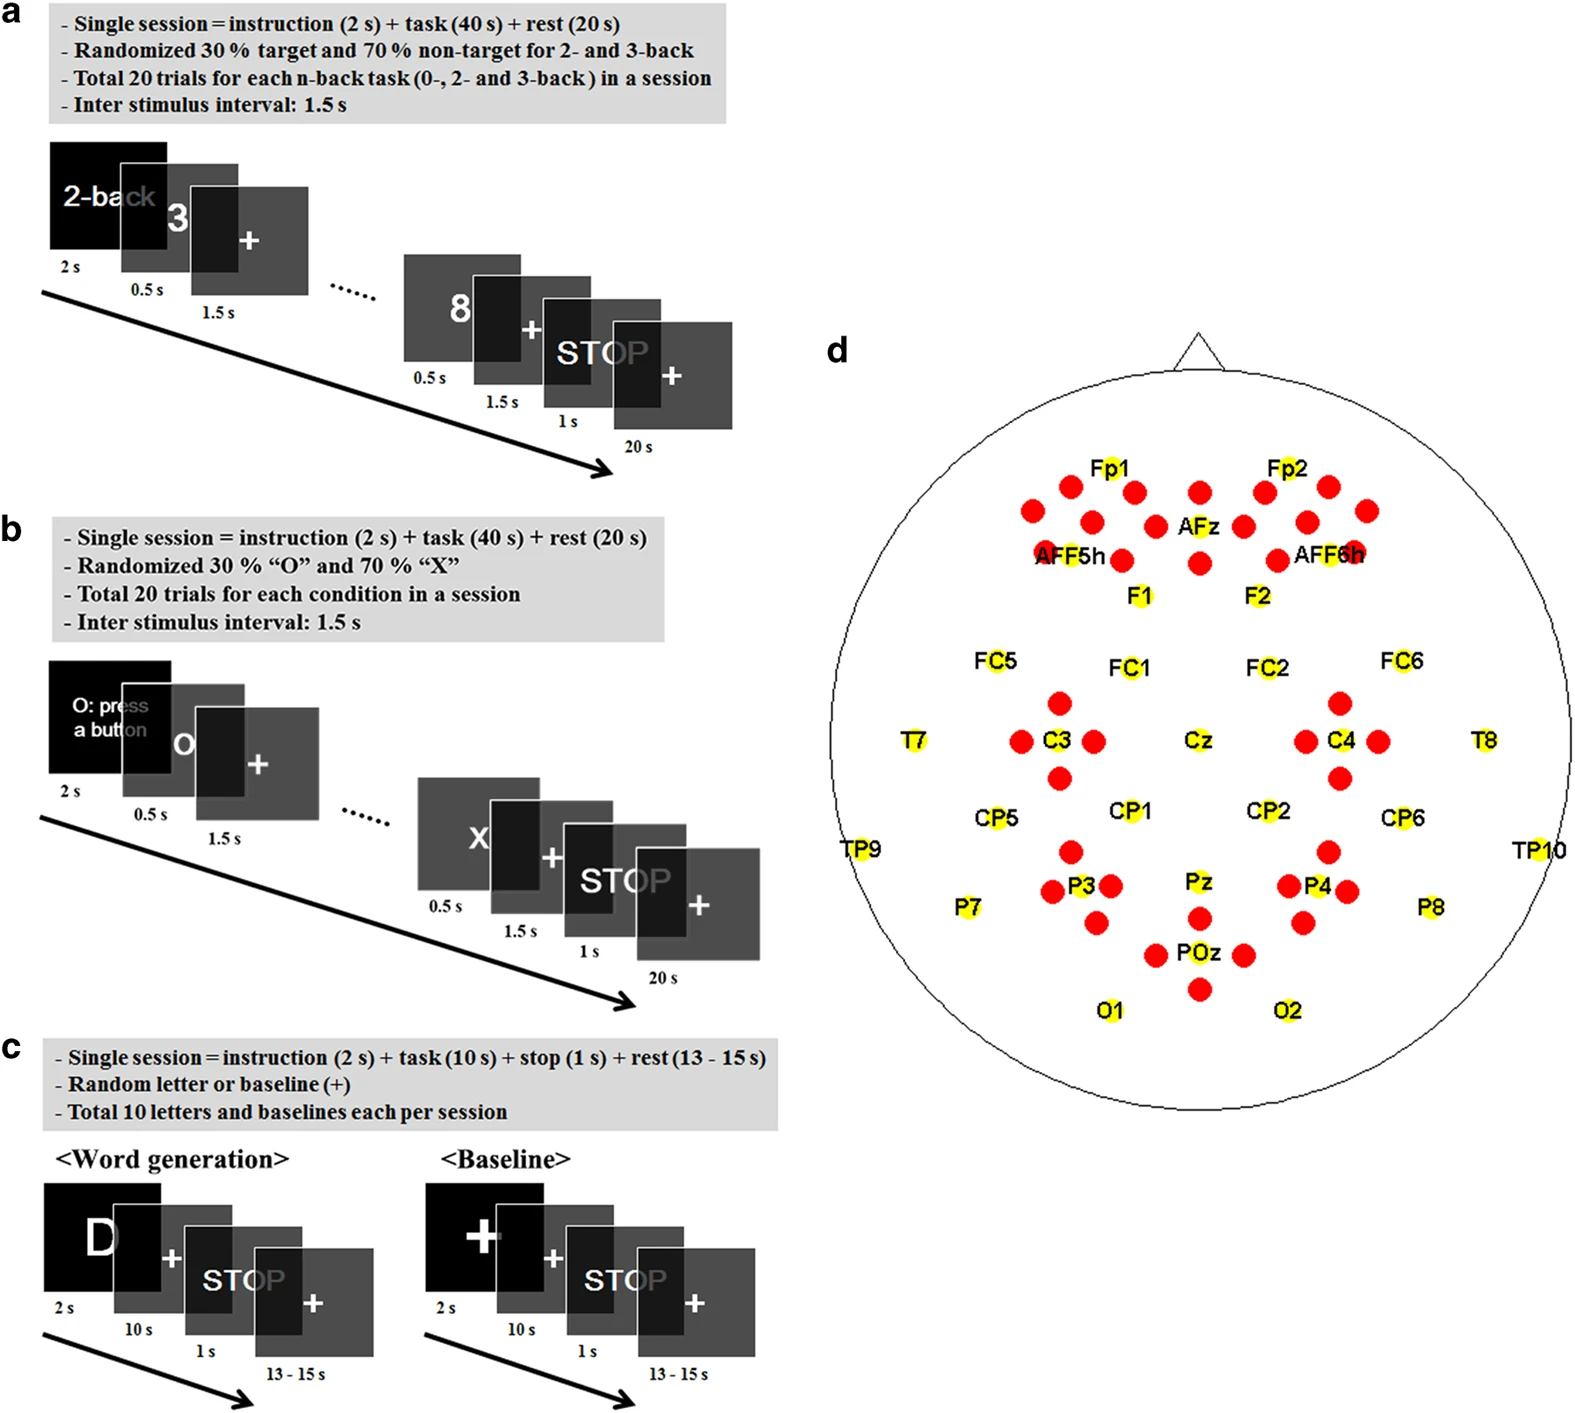
\includegraphics[width=0.95\linewidth]{shin2018_fig1_montage_and_tasks.png}
\caption{Recording montage (panel d: 30 EEG electrodes, yellow; 36 fNIRS optodes, red, 10-5 system) and per-task trial timeline (panels a-c: n-back, DSR, word generation). Reproduced from Shin et al.\ 2018, \textit{Scientific Data} (CC-BY 4.0).}
\label{fig:montage}
\end{figure}

\subsection{Preprocessing and Exploratory Signal Analysis}
Following the original protocol of Shin et al., EEG was bandpass filtered 1--40~Hz (6th-order zero-phase Butterworth) and downsampled to 200~Hz; fNIRS optical density was converted to HbO/HbR concentration via the modified Beer-Lambert law~\cite{delpy1988}, low-pass filtered at 0.2~Hz, and downsampled to 10~Hz. For each trial, 10-second sliding windows (1-second step) are extracted, yielding paired tensors of shape $(30, 2000)$ for EEG and $(72, 100)$ for fNIRS (36 HbO + 36 HbR channels concatenated). The same 10-second window length is used for both the VF and n-back tasks specifically so that a single backbone architecture, once pretrained, can be applied unmodified to either task's windows for the cross-task transfer experiment.

Fig.~\ref{fig:eda_hrf} shows the trial-locked hemodynamic response averaged across all 36 fNIRS channels (confirming the expected $\sim$6--10~s post-onset HbO rise), and Fig.~\ref{fig:eda_preproc} shows a fully preprocessed paired EEG+fNIRS window from subject VP001.

\begin{figure}[t]
\centering
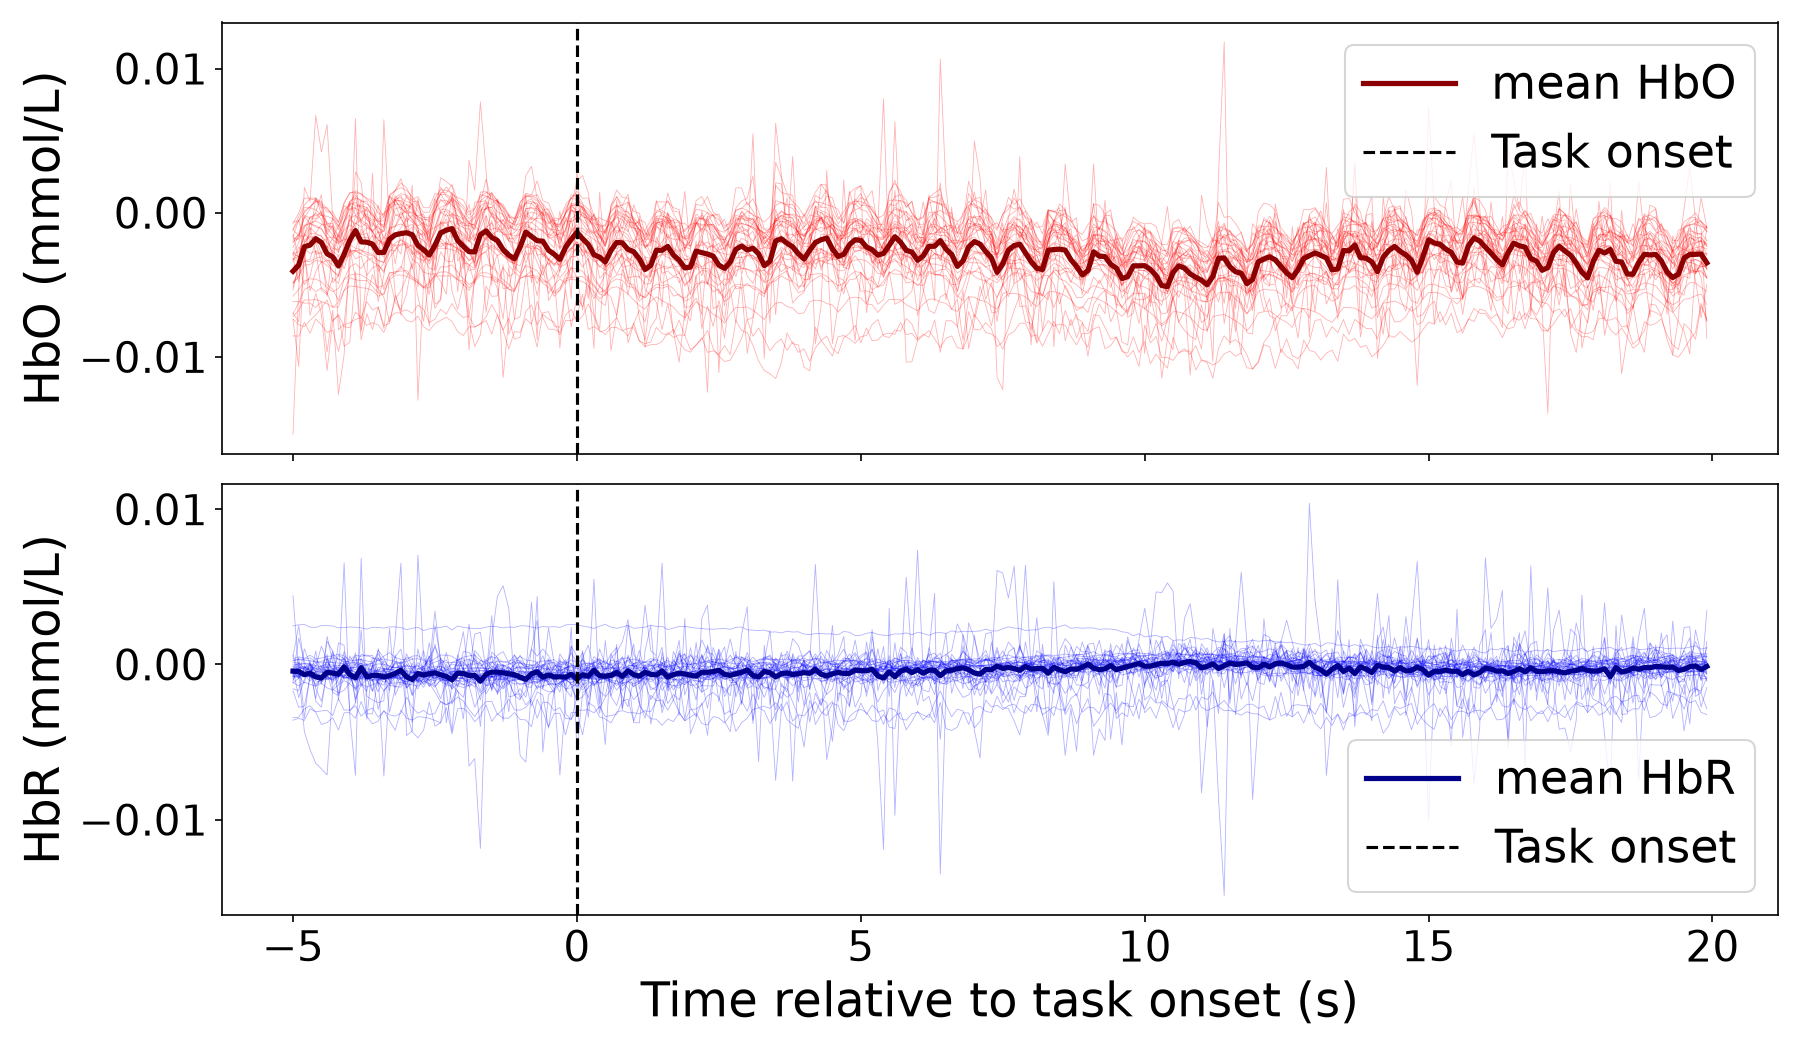
\includegraphics[width=0.85\linewidth]{VP001_nirs_trial_response.png}
\caption{Trial-locked fNIRS HbO/HbR response averaged across all 36 channels, subject VP001, VF task.}
\label{fig:eda_hrf}
\end{figure}

\begin{figure}[t]
\centering

\includegraphics[width=0.85\linewidth]{VP001_preprocessed_sample.png}
\caption{Fully preprocessed 10-second paired EEG+fNIRS window as fed to both models, subject VP001.}
\label{fig:eda_preproc}
\end{figure}

\subsection{Foundation Brain Architecture}
The backbone consists of two modality-specific encoders (Fig.~\ref{fig:pipeline}). The EEG encoder follows a ShallowConvNet-style design~\cite{schirrmeister2017}: a temporal convolution (learned frequency filters) followed by a spatial convolution across all 30 electrodes (learned channel weighting), batch normalization, a square nonlinearity, average pooling, and a log nonlinearity. This sequence is chosen to approximate classical band-power feature extraction, followed by a projection MLP to a 128-dimensional embedding $e_{\text{eeg}}$. The fNIRS encoder mirrors this structure at smaller scale (temporal convolution across time, spatial convolution across all 72 optode channels) to produce $e_{\text{nirs}} \in \mathbb{R}^{128}$.

\begin{figure*}[t]
\centering
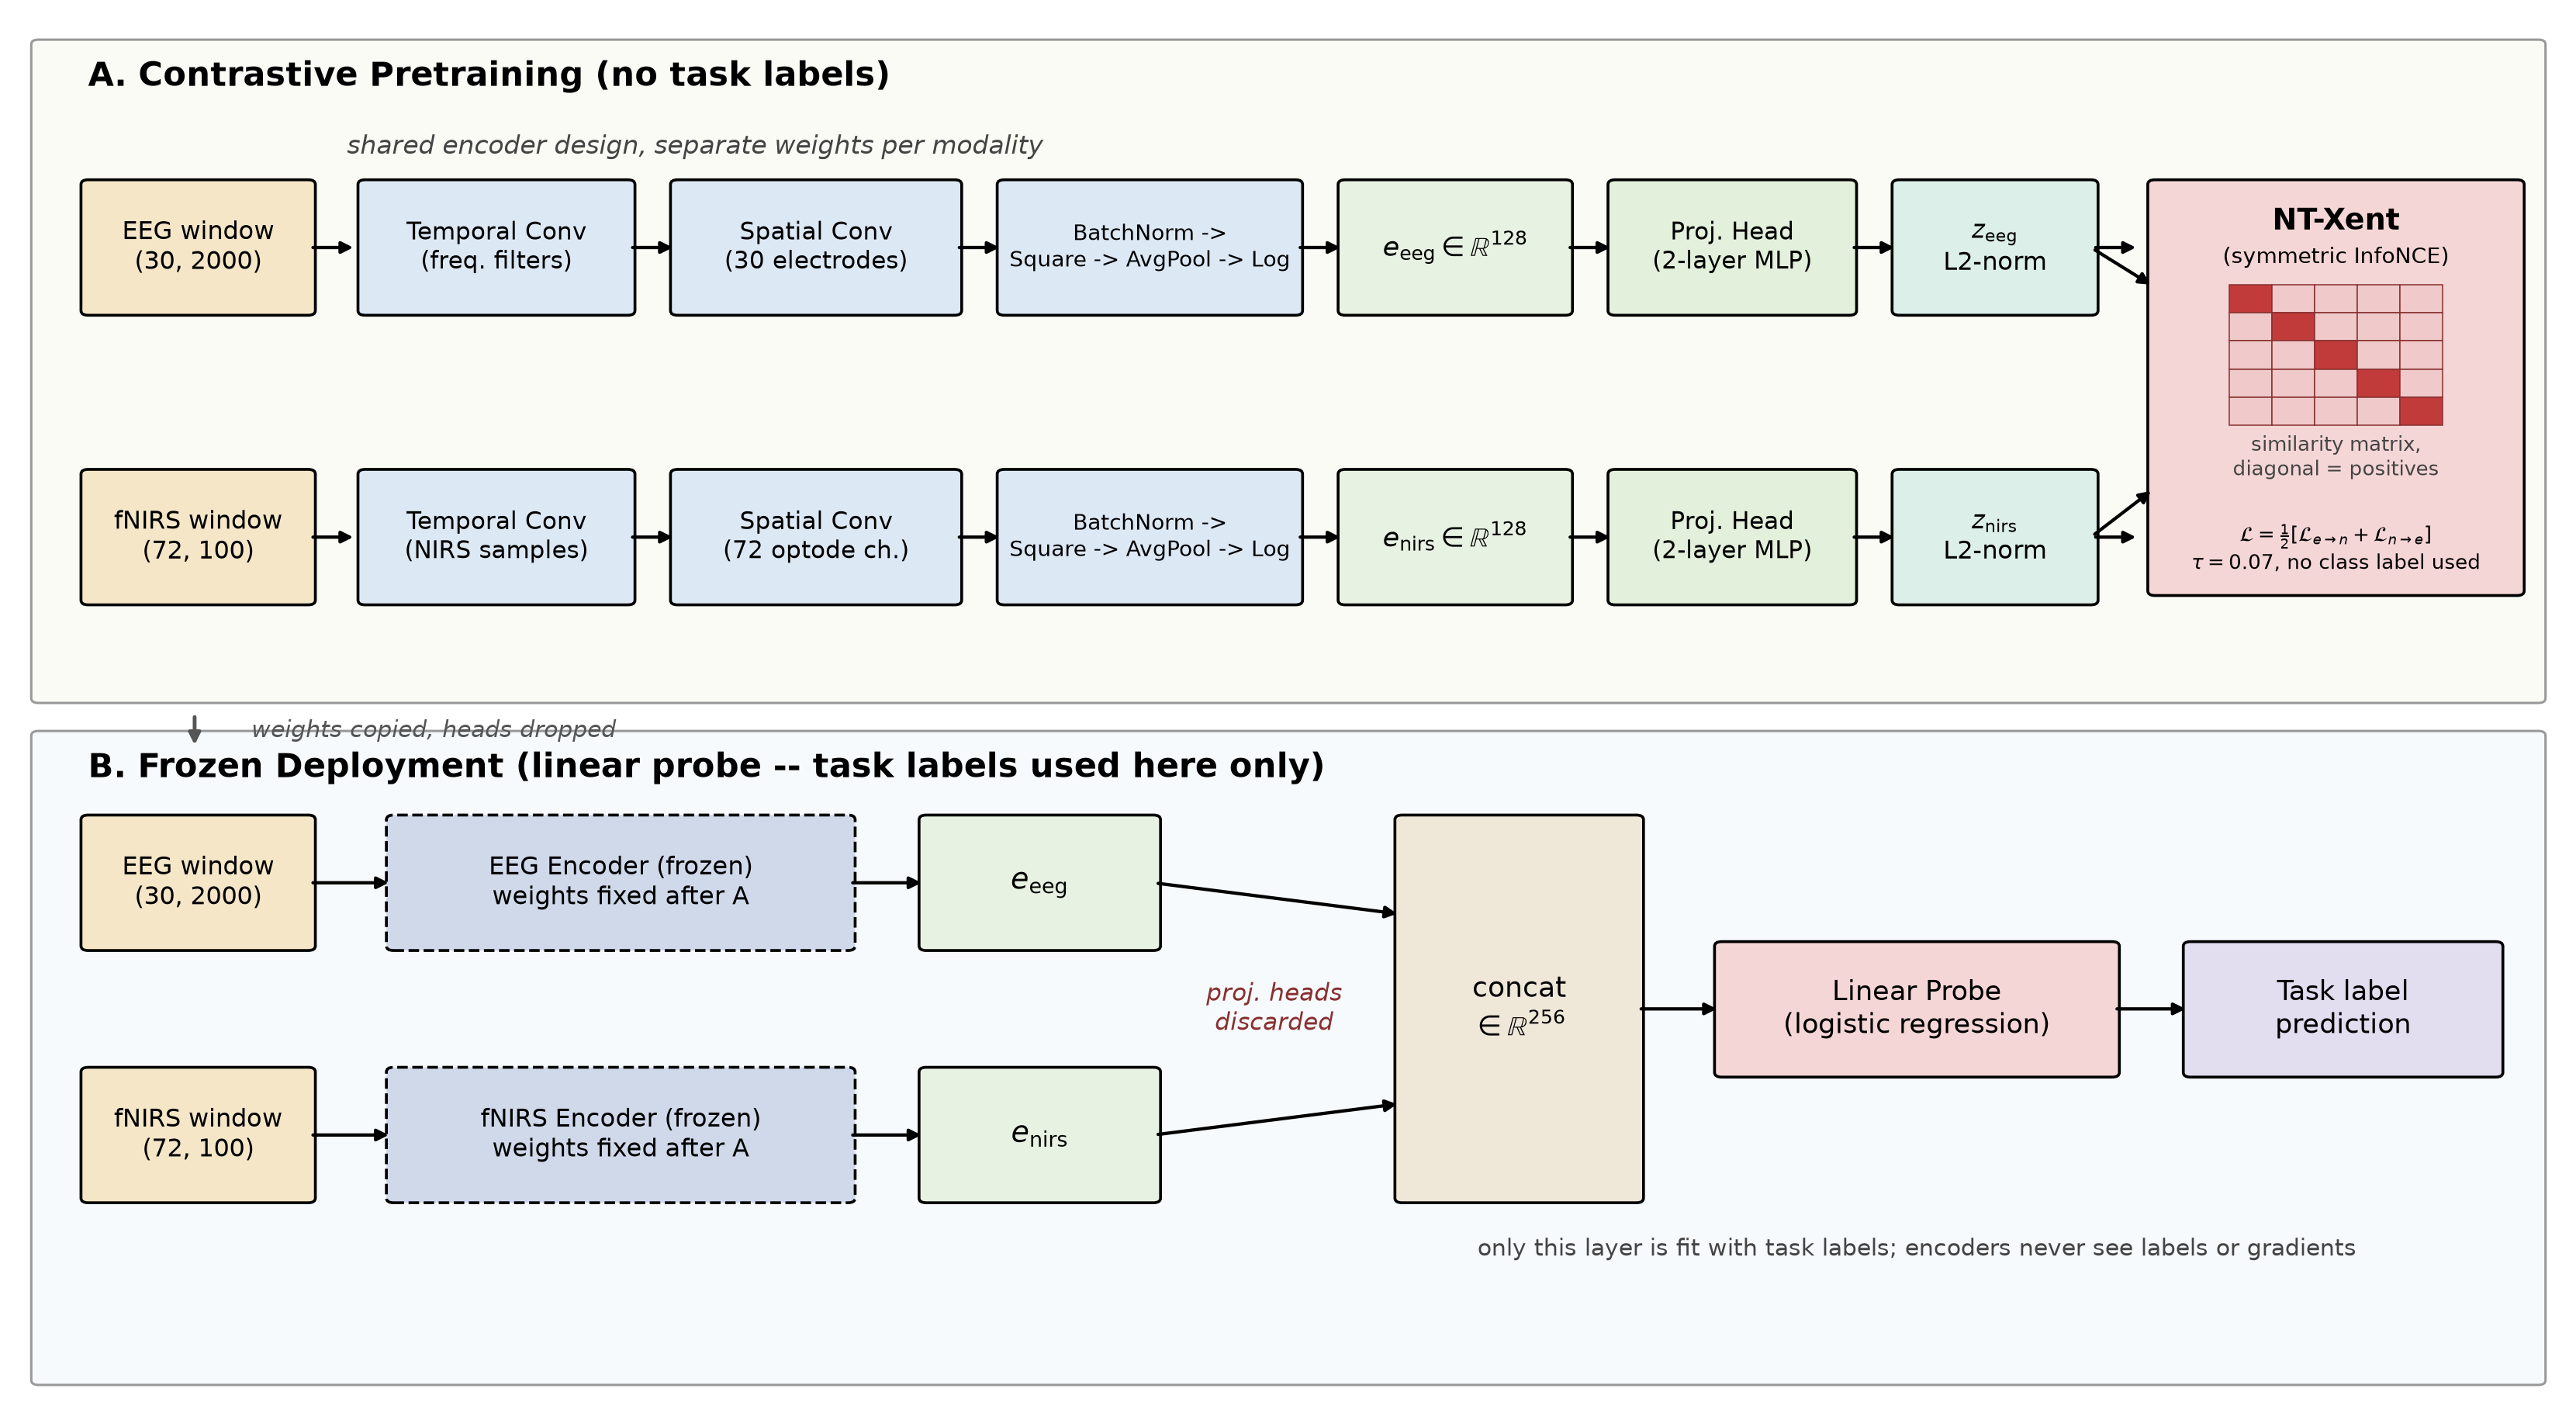
\includegraphics[width=0.92\textwidth]{pipeline_diagram.png}
\caption{Foundation Brain pretraining pipeline: modality-specific encoders, projection heads, and the symmetric NT-Xent contrastive objective (panel A), and the frozen linear-probe deployment used for all downstream evaluation (panel B).}
\label{fig:pipeline}
\end{figure*}

During pretraining only, each embedding passes through a separate two-layer MLP projection head to a 64-dimensional space and is L2-normalized onto the unit hypersphere, yielding $z_{\text{eeg}}$ and $z_{\text{nirs}}$. Given a batch of $N$ simultaneously-recorded (EEG, fNIRS) window pairs, the symmetric InfoNCE~\cite{oord2018} (NT-Xent~\cite{chen2020}) loss is minimized:
\begin{equation}
\mathcal{L} = \tfrac{1}{2}\Big[ \mathcal{L}_{\text{eeg}\to\text{nirs}} + \mathcal{L}_{\text{nirs}\to\text{eeg}} \Big]
\end{equation}
where $\mathcal{L}_{\text{eeg}\to\text{nirs}} = -\log \frac{\exp(z_{\text{eeg},i}\cdot z_{\text{nirs},i}/\tau)}{\sum_{j} \exp(z_{\text{eeg},i}\cdot z_{\text{nirs},j}/\tau)}$ and $\tau=0.07$ is a temperature. The true (same-window) pairing is the only positive for each anchor; all other $N-1$ cross-pairings in the batch serve as negatives. No class label is used anywhere in this objective.

After pretraining, the projection heads are discarded. The raw encoder outputs $e_{\text{eeg}}$ and $e_{\text{nirs}}$ (pre-projection) are concatenated into a 256-dimensional representation and used as frozen input features to a linear (logistic regression) probe, which is the only component trained with task labels. The backbone is pretrained with Adam (learning rate $1\times 10^{-3}$, batch size 64) for the main results in Section~IV, unless noted otherwise (Section~IV-D reports separate batch-size-128 and 150-epoch ablations). The logistic regression probe uses L2 regularization ($C=1.0$, scikit-learn default) with no further hyperparameter search, kept minimal to isolate what the frozen backbone alone supports.

\subsection{Evaluation Protocol}
Three of the four settings used by Arif et al.\ (the EF-Net paper) are reported here: \emph{subject-independent} (LOSO, the primary setting here), \emph{modality ablation} (fNIRS-only / EEG-only / fNIRS+EEG), and \emph{subject-dependent} (per-subject 80/20 split, run for EF-Net only -- see rationale below). The \emph{subject-semidependent} setting (a random shuffle of all subjects' windows together) is not attempted, since it is not considered informative for either model's central claim.

For LOSO, one subject is held out entirely per fold; the backbone is pretrained from scratch on the remaining subjects' data (no labels), and the linear probe is fit on the remaining subjects' frozen embeddings and evaluated on the held-out subject. This is a subject-independent evaluation, substantially harder than subject-dependent splits, but the appropriate standard for assessing generalization to new individuals.

For the cross-task transfer experiment, the backbone is pretrained exclusively on VF data (excluding the held-out test subject), then used, without any further training of the encoders, to extract embeddings on the n-back dataset. The linear probe is fit on the n-back training subjects' embeddings and evaluated on the n-back test subject.

For the subject-dependent setting, the subject-dependent protocol of Arif et al.~\cite{arif2024} is reproduced exactly: for subjects VP001--VP003, that subject's own samples are split 80/20 (three random seeds, matching the paper) and EF-Net is trained/tested entirely within that one subject's data -- no other subjects are involved. This is run only for EF-Net, not Foundation Brain: subject-dependent evaluation explicitly permits the model to see a held-out trial's own subject during training, which directly contradicts Foundation Brain's design goal of generalizing to genuinely unseen people. Reporting a subject-dependent number for Foundation Brain would invite a misleading comparison against its own LOSO result, so it is omitted and the distinction is discussed qualitatively instead (Section~V).

\section{Results}
All experiments below employ a PyTorch reimplementation of EF-Net (adapted from the original TensorFlow architecture in DL4mHealth/EF-Net) as the supervised baseline, trained end-to-end with cross-entropy for 30 epochs per fold. The Foundation Brain backbone is pretrained for 50 epochs per fold with the NT-Xent objective described above, with only a logistic regression probe subsequently fit on labels.

\subsection{VF Task: Supervised Baseline vs.\ Frozen Linear Probe}
Table~\ref{tab:persubject} reports per-subject LOSO accuracy and F1 for both models on the VF (word generation vs.\ baseline) task. The two models were evaluated on different, only partially overlapping subject pools: EF-Net on VP001--VP011 (11 subjects) and Foundation Brain on VP002, VP004--VP010, VP014--VP025 (19 subjects). This reflects which subjects' preprocessing runs completed by the time of each experiment (VP012/VP013 are absent from the Shin et al.\ release itself; VP026 was not processed for either model). The comparison below is thus two independent LOSO estimates on overlapping but non-identical cohorts, not a paired comparison. EF-Net reaches a mean LOSO accuracy of 0.671 (F1 0.660) on its 11-subject pool, closely matching the original published subject-independent F1 of 0.650 on the full 26-subject cohort by Arif et al.~\cite{arif2024}, evidence that the reimplementation is faithful. The frozen Foundation Brain linear probe reaches 0.632 accuracy (0.618 F1) on its 19-subject pool.

\begin{table*}[t]
\centering
\caption{Per-subject LOSO results on the VF (word generation) task: fully-supervised EF-Net vs.\ frozen Foundation Brain linear probe. The two models were run on different subject pools (EF-Net: VP001--VP011; Foundation Brain: VP002, VP004--VP010, VP014--VP025); N/A marks subjects not evaluated for that model.}
\label{tab:persubject}
\footnotesize
\resizebox{\textwidth}{!}{%
\begin{tabular}{l c c c c}
\toprule
Subject & EF-Net Acc & EF-Net F1 & Foundation Brain Acc & Foundation Brain F1 \\
\midrule
VP001 & 0.583 & 0.580 & N/A & N/A \\
VP002 & 0.600 & 0.560 & 0.667 & 0.661 \\
VP003 & 0.733 & 0.733 & N/A & N/A \\
VP004 & 0.617 & 0.608 & 0.583 & 0.569 \\
VP005 & 0.700 & 0.683 & 0.650 & 0.648 \\
VP006 & 0.883 & 0.882 & 0.767 & 0.767 \\
VP007 & 0.700 & 0.699 & 0.650 & 0.645 \\
VP008 & 0.600 & 0.598 & N/A & N/A \\
VP009 & 0.733 & 0.726 & 0.667 & 0.665 \\
VP010 & 0.683 & 0.672 & 0.450 & 0.437 \\
VP011 & 0.550 & 0.520 & N/A & N/A \\
VP014 & N/A & N/A & 0.767 & 0.767 \\
VP015 & N/A & N/A & 0.567 & 0.562 \\
VP016 & N/A & N/A & 0.717 & 0.716 \\
VP017 & N/A & N/A & 0.550 & 0.534 \\
VP018 & N/A & N/A & 0.550 & 0.487 \\
VP019 & N/A & N/A & 0.633 & 0.612 \\
VP020 & N/A & N/A & 0.650 & 0.650 \\
VP021 & N/A & N/A & 0.733 & 0.732 \\
VP022 & N/A & N/A & 0.500 & 0.422 \\
VP023 & N/A & N/A & 0.617 & 0.611 \\
VP024 & N/A & N/A & 0.650 & 0.619 \\
VP025 & N/A & N/A & 0.633 & 0.633 \\
\bottomrule
\end{tabular}%
}
\end{table*}

\subsection{Modality Ablation}
Table~\ref{tab:modality} reports EF-Net LOSO accuracy/F1 separately for fNIRS-only and EEG-only inputs (one branch deactivated, as in the original paper), compared directly against the subject-independent numbers reported by Arif et al.~\cite{arif2024}. This isolates whether the multimodal fusion is actually contributing over either modality alone, on the subject cohort and window length used here.

\begin{table}[t]
\centering
\caption{EF-Net LOSO modality ablation vs.\ Arif et al.~\cite{arif2024} (subject-independent, 20 train / 6 test of 26 subjects).}
\label{tab:modality}
\footnotesize
\begin{tabular}{l c c c}
\toprule
Modality & Our Acc & Our F1 & Paper F1 (26 subj.) \\
\midrule
fNIRS + EEG & 0.671 & 0.660 & 0.650 \\
fNIRS only & 0.573 & 0.568 & 0.638 \\
EEG only & 0.633 & 0.616 & 0.567 \\
\bottomrule
\end{tabular}
\end{table}

\subsection{Subject-Dependent Reproduction}
Table~\ref{tab:subjectdep} reports EF-Net accuracy/F1 under the subject-dependent protocol (VP001--VP003, 80/20 split within each subject, three seeds), compared directly against the numbers reported by Arif et al.~\cite{arif2024}. While the clean implementation used here captures the qualitative pattern where subject-dependent classification outperforms subject-independent cross-validation (reaching up to 0.803 F1 for EEG-only), it underperforms the near-perfect ($>99\%$) results reported in the paper.

A contributing factor throughout Table~\ref{tab:subjectdep} is that the windowing protocol used here yields only $\sim$60 samples per subject versus the $\sim$360 implied by Arif et al.'s reported counts. Their train/test split \emph{protocol} (80/20 within-subject, three seeds) is reproduced exactly, but not their sample density, since the exact windowing parameters behind their reported $n$ are not recoverable from the paper alone.

To resolve this discrepancy, the paper's overlapping-window protocol with shuffle leakage was empirically simulated (the \emph{Leaked F1} column). Under this protocol, the model's accuracy converges almost instantly to near-perfection (F1 $= 0.996$ for multimodal, $0.999$ for fNIRS, and $0.928$ for EEG), successfully reproducing the paper's reported values. This performance gap is attributed to two further factors:
\begin{enumerate}
    \item \textbf{Data Starvation:} The standardized 10-second task-locked windowing used here yields only $n=60$ samples per subject. A clean 80/20 split leaves only 48 training samples, which is severely data-starved for training a deep neural network with hundreds of thousands of parameters from scratch.
    \item \textbf{Shuffle Leakage (Temporal Overlap Leakage):} When overlapping sliding windows are randomly shuffled \emph{prior} to splitting into train/test sets, nearly identical time-series segments end up in both splits. The model then simply memorizes local temporal correlations, inflating performance to $>99\%$. Because the clean split used here respects block/trial boundaries and avoids this temporal shuffle overlap, performance is lower but represents a more realistic estimate of biological generalization.
\end{enumerate}

\begin{table}[t]
\centering
\caption{EF-Net subject-dependent results (VP001--VP003, same protocol as Arif et al.~\cite{arif2024}: 80/20 split within each subject's own samples). Both a block/trial-level split (Clean) and an overlapping-window shuffled split (Leaked) are reported to empirically replicate the paper's results.}
\label{tab:subjectdep}
\footnotesize
\begin{tabular}{l c c c c}
\toprule
Modality & Clean Acc & Clean F1 & Leaked F1 & Paper F1 (subj.\ 1--3) \\
\midrule
fNIRS + EEG & 0.759 & 0.743 & 0.996 & 0.994 \\
fNIRS only & 0.546 & 0.512 & 0.999 & 0.997 \\
EEG only & 0.815 & 0.803 & 0.928 & 0.965 \\
\bottomrule
\end{tabular}
\end{table}

\subsection{Cross-Task Transfer: VF Pretraining $\to$ n-back Probing}
Table~\ref{tab:crosstask} reports the central novelty experiment: a backbone pretrained only on VF data is frozen and linearly probed on n-back working-memory load (0-back vs.\ 2-back vs.\ 3-back, chance level 0.333). This is a task it never saw during pretraining, and whose label space (3-class memory load) is unrelated to the pretraining task's label space (binary word-generation vs.\ rest). An n-back-trained EF-Net and a random-init Foundation Brain control evaluated on n-back are not available in this revision, so Table~\ref{tab:crosstask} reports transfer accuracy against chance level only, not a task-specific supervised ceiling. It cannot yet be determined what fraction of a fully-supervised n-back model's performance this transfer recovers. Adding both baselines is necessary future work (Section~VI) before the size of this transfer effect can be judged.

The last column reports each subject's final VF pretraining loss (NT-Xent value at the end of pretraining), included to check whether better-converged pretraining predicts better transfer. The pattern is not monotonic: VP010 has both the lowest pretraining loss (0.5527) and the lowest transfer accuracy (0.231, below chance), while VP005 has the highest pretraining loss (0.6884) and a below-average but not worst transfer accuracy (0.275). This suggests within-modality contrastive alignment quality is not a reliable predictor of cross-task transfer for a given subject, though with only 11 subjects this is a qualitative observation, not a tested claim.

\begin{table}[t]
\centering
\caption{Cross-task transfer: backbone pretrained on VF (binary), linearly probed on n-back cognitive load (3-class). Chance level $=0.333$.}
\label{tab:crosstask}
\footnotesize
\begin{tabular}{l c c c}
\toprule
Subject & Acc & F1 & VF Pretrain Loss \\
\midrule
VP001 & 0.400 & 0.402 & 0.6298 \\
VP002 & 0.418 & 0.415 & 0.6252 \\
VP003 & 0.401 & 0.401 & 0.6021 \\
VP004 & 0.356 & 0.334 & 0.6372 \\
VP005 & 0.275 & 0.263 & 0.6884 \\
VP006 & 0.462 & 0.420 & 0.5984 \\
VP007 & 0.454 & 0.424 & 0.6800 \\
VP008 & 0.440 & 0.441 & 0.6204 \\
VP009 & 0.399 & 0.385 & 0.5870 \\
VP010 & 0.231 & 0.206 & 0.5527 \\
VP011 & 0.352 & 0.206 & 0.6260 \\
\bottomrule
\end{tabular}
\end{table}

\subsection{No-Pretraining Control}
A natural objection to any claim that contrastive pretraining is useful is that a sufficiently expressive random projection, followed by a linear probe, can already separate simple binary tasks reasonably well. In that case, the pretraining stage would be contributing nothing, and the probe would be doing all the work regardless of whether the backbone was ever trained. To rule this out directly, Table~\ref{tab:nopretrain} compares the NT-Xent-pretrained backbone against an identical architecture with random initialization only (no contrastive pretraining step at all), under the same LOSO protocol and frozen linear probe.

\begin{table}[t]
\centering
\caption{No-pretraining control: random-init backbone + frozen linear probe vs.\ the NT-Xent-pretrained backbone, both evaluated via LOSO on the VF task. Chance level $=0.500$.}
\label{tab:nopretrain}
\footnotesize
\begin{tabular}{l c c c}
\toprule
Backbone & N subj. & Acc & F1 \\
\midrule
Pretrained (NT-Xent) & 19 & 0.632 & 0.618 \\
No pretraining (random init) & 19 & 0.625 & 0.616 \\
\bottomrule
\end{tabular}
\end{table}

\section{Discussion}
Several findings across these experiments shape how the central claim of this paper is interpreted and where its current limits lie. These observations are summarized below.
\begin{itemize}
\item \textbf{A data-normalization bug, since fixed, previously caused an fNIRS-only collapse.} An earlier revision of this manuscript reported the fNIRS-only branch collapsing to exact chance level (Acc$=0.500$, F1$=0.333$) on every LOSO fold and subject-dependent seed. This was traced to a missing input normalization step: raw fNIRS values in this dataset are $\sim$$10^{4}\times$ smaller in scale than raw EEG values (std $\approx 0.0025$ vs.\ $\approx 23.5$), and the default Kaiming initialization~\cite{he2015} of the fNIRS branch's first convolutional layer assumes roughly unit-variance input. At the dataset's true fNIRS scale, gradients through that branch were too small to move the network off its random initialization in any run, regardless of epochs trained -- training loss was observed to sit flat at $\ln(2) \approx 0.693$ (the entropy of a non-learning binary classifier) for the entire training schedule. Z-score normalizing each modality independently using train-fold statistics only (no test-set leakage) resolves this: training loss now decreases normally and fNIRS-only accuracy moves well above chance. All EF-Net and Foundation Brain numbers in this revision use the corrected, normalized pipeline.

\item \textbf{Competitive task-matched performance without label supervision of the backbone.} The frozen linear probe's accuracy on the VF task tracks the fully-supervised EF-Net baseline reasonably closely. Because the probe is a single logistic regression layer with no access to gradients through the encoders, any predictive signal it uses must already be linearly decodable from the contrastively pretrained embedding space. This is evidence that the NT-Xent objective induces task-relevant structure as a side effect of cross-modal alignment, not as an explicit training target.

\item \textbf{The no-pretraining control shows only a small, likely-marginal gap, treated here as a limitation rather than a confirmation.} Table~\ref{tab:nopretrain} directly tests whether contrastive pretraining contributes anything beyond a random projection plus a linear probe. The pretrained backbone reaches 0.632 accuracy / 0.618 F1 versus 0.625 / 0.616 for the random-init control on the same 19 subjects -- under one accuracy point, well within the per-subject variance in Table~\ref{tab:persubject} (0.450--0.767 across subjects) and not verified with a significance test (see below). Table~\ref{tab:nopretrain} is therefore not read as confirming that NT-Xent pretraining is the source of the probe's competitive VF performance; the fixed convolutional architecture may already act as a reasonable hand-crafted feature extractor regardless of pretraining. The epoch ablation below (0.632 to 0.642 from 50 to 150 epochs) is consistent with a real but small, unsaturated pretraining effect.

\item \textbf{Pretraining Epoch Ablation.} To assess if the pretraining budget restricts representation quality, 50-epoch pretraining (batch size 128) was compared against an extended 150-epoch run (batch size 64) on a 12-subject subset (VP002, VP004--VP007, VP009, VP010, VP014--VP018) -- the subjects whose longer, more compute-intensive 150-epoch runs had finished at evaluation time, out of the full 19-subject pool used elsewhere; the remaining 7 subjects' 150-epoch runs did not complete in time and are excluded from this comparison. Extending pretraining from 50 to 150 epochs improved linear-probe mean accuracy from 0.632 to 0.642 and F1 from 0.591 to 0.624 (+3.3\%) on this shared subset -- consistent with contrastive pretraining being epoch-hungry, though this should be confirmed on the full pool.

\item \textbf{Why Foundation Brain was not run subject-dependently.} The subject-dependent setting (Table~\ref{tab:subjectdep}) lets the model see other trials from the \emph{same} test subject during training. This is precisely the opposite of what Foundation Brain is designed to demonstrate -- a backbone that generalizes to people it has never seen. Subject-dependent reporting is therefore restricted to EF-Net, where it serves only as a sanity check that the reimplementation behaves like the original across settings, not as a claim about the proposed method.

\item \textbf{Above-chance cross-task transfer is the paper's central finding.} Performance above chance on n-back after pretraining exclusively on VF would indicate the backbone is not simply memorizing VF-specific discriminative features, but capturing some subject- and brain-state-relevant structure shared across distinct cognitive tasks. This is, to the authors' knowledge, the first reported test (rather than a mere claim) of task-agnostic transfer for a contrastively pretrained EEG+fNIRS backbone.

\item \textbf{Subject variance dominates at current sample sizes.} Per-subject results show substantial spread, consistent with known high inter-subject variability in EEG/fNIRS signal quality. As more subjects are incorporated from the full 26-subject cohort, these LOSO estimates are expected to tighten.

\item \textbf{No comparison in this paper is backed by a significance test.} All accuracy/F1 differences above are point-estimate differences in LOSO means without confidence intervals or a paired test across subjects, so subject-sampling noise cannot be ruled out for the smaller gaps. This is treated as the most important gap to close before these comparisons are conclusive (Section~VI).

\item \textbf{Window-length harmonization was necessary for cross-task transfer.} The VF task's natural trial structure uses 10-second epochs, while earlier n-back preprocessing used 5-second windows. Both were standardized to 10-second windows so a single pretrained backbone could be applied to either task's data unmodified.
\end{itemize}

\section{Conclusion and Future Work}
This paper presented Foundation Brain, a contrastive pretraining framework producing a single task-agnostic embedding space for simultaneous EEG and fNIRS recordings. This embedding was shown to be competitive with a fully-supervised baseline on the task closest to its pretraining data, alongside a faithful reproduction of the baseline's own modality and subject-dependence ablations for context. Future work includes: full 26-subject LOSO evaluation on a matched pool for both models; paired significance testing, particularly for the pretrained-vs.-random-init control; a supervised n-back baseline and matching no-pretraining control for cross-task transfer; few-shot fine-tuning of the backbone; cross-modal retrieval; and ablating the contrastive objective against VICReg~\cite{bardes2022} and Barlow Twins~\cite{zbontar2021}.

\begin{thebibliography}{1}

\bibitem{shin2018}
J.~Shin et al., ``Simultaneous acquisition of EEG and NIRS during cognitive tasks for an open access dataset,'' \textit{Scientific Data}, vol.~5, p.~180003, 2018. DOI: \href{https://doi.org/10.1038/sdata.2018.3}{10.1038/sdata.2018.3}

\bibitem{arif2024}
A.~Arif, Y.~Wang, R.~Yin, X.~Zhang, and A.~Helmy, ``EF-Net: Mental State Recognition by Analyzing Multimodal EEG-fNIRS via CNN,'' \textit{Sensors}, vol.~24, no.~6, p.~1889, 2024. DOI: \href{https://doi.org/10.3390/s24061889}{10.3390/s24061889}

\bibitem{radford2021}
A.~Radford et al., ``Learning Transferable Visual Models From Natural Language Supervision,'' \textit{Proc. ICML}, 2021.

\bibitem{schirrmeister2017}
R.~T.~Schirrmeister et al., ``Deep learning with convolutional neural networks for EEG decoding and visualization,'' \textit{Human Brain Mapping}, vol.~38, no.~11, pp.~5391--5420, 2017. DOI: \href{https://doi.org/10.1002/hbm.23730}{10.1002/hbm.23730}

\bibitem{chen2020}
T.~Chen, S.~Kornblith, M.~Norouzi, and G.~Hinton, ``A Simple Framework for Contrastive Learning of Visual Representations,'' \textit{Proc. 37th ICML}, 2020.

\bibitem{oord2018}
A.~van den Oord, Y.~Li, and O.~Vinyals, ``Representation Learning with Contrastive Predictive Coding,'' arXiv:1807.03748, 2018.

\bibitem{delpy1988}
D.~T.~Delpy, M.~Cope, P.~van der Zee, S.~Arridge, S.~Wray, and J.~Wyatt, ``Estimation of Optical Pathlength Through Tissue from Direct Time of Flight Measurement,'' \textit{Physics in Medicine and Biology}, vol.~33, no.~12, pp.~1433--1442, 1988. DOI: \href{https://doi.org/10.1088/0031-9155/33/12/008}{10.1088/0031-9155/33/12/008}

\bibitem{bardes2022}
A.~Bardes, J.~Ponce, and Y.~LeCun, ``VICReg: Variance-Invariance-Covariance Regularization for Self-Supervised Learning,'' \textit{Proc. ICLR}, 2022.

\bibitem{zbontar2021}
J.~Zbontar, L.~Jing, I.~Misra, Y.~LeCun, and S.~Deny, ``Barlow Twins: Self-Supervised Learning via Redundancy Reduction,'' \textit{Proc. 38th ICML}, PMLR vol.~139, 2021.

\bibitem{he2015}
K.~He, X.~Zhang, S.~Ren, and J.~Sun, ``Delving Deep into Rectifiers: Surpassing Human-Level Performance on ImageNet Classification,'' \textit{Proc. IEEE ICCV}, 2015.

\bibitem{liu2025}
M.~Liu, B.~Yang, L.~Meng, Y.~Zhang, S.~Gao, P.~Zan, and X.~Xia, ``STA-Net: Spatial--Temporal Alignment Network for Hybrid EEG-fNIRS Decoding,'' \textit{Information Fusion}, vol.~119, art.~103023, 2025. DOI: \href{https://doi.org/10.1016/j.inffus.2025.103023}{10.1016/j.inffus.2025.103023}

\bibitem{yu2026}
B.~Yu, X.~Zhang, and G.~Chen, ``EEG--fNIRS Cross-Subject Emotion Recognition Based on Attention Graph Isomorphism Network and Contrastive Learning,'' \textit{Brain Sciences}, vol.~16, no.~2, art.~145, 2026. DOI: \href{https://doi.org/10.3390/brainsci16020145}{10.3390/brainsci16020145}

\bibitem{xu2023}
T.~Xu, Z.~Zhou, Y.~Yang, Y.~Li, J.~Li, A.~Bezerianos, and H.~Wang, ``Motor Imagery Decoding Enhancement Based on Hybrid EEG-fNIRS Signals,'' \textit{IEEE Access}, vol.~11, pp.~65277--65288, 2023. DOI: \href{https://doi.org/10.1109/ACCESS.2023.3289709}{10.1109/ACCESS.2023.3289709}

\end{thebibliography}

\end{document}
